\chapter{Analisis Masalah}
\label{chap:analisis}

Pada bab ini akan dibahas survei kesalahan umum dan keputusan implementasi hasil survei.

\section{Survei Kesalahan Umum}
\label{sec:survei}

Pada bagian ini akan dijelaskan tentang survei yang dilakukan untuk mengumpulkan informasi yang dibutuhkan dalam pengembangan perangkat lunak. Informasi yang dicari adalah tentang kesalahan-kesalahan umum yang sering terjadi pada penulisan dokumen skripsi. Untuk mengumpulkan informasi tersebut, metode yang dipilih adalah melakukan survei. Dalam pelaksanaannya, survei dibagi menjadi dua, yaitu pengamatan beberapa sidang skripsi dan wawancara secara personal kepada dosen-dosen Informatika Unpar. 

\subsection{Pengamatan Sidang}
Pengamatan dilakukan pada sidang skripsi semester Ganjil 2018/2019, yang berlangsung pada bulan Mei 2019. Tidak semua sidang skripsi yang berlangsung diamati, melainkan dari 42 sidang skripsi hanya diambil 7 sidang skripsi saja. Hal tersebut dilakukan dengan pertimbangan dari ke-7 sidang skripsi tersebut diuji oleh dosen Informatika yang berbeda-beda. Namun ada beberapa dosen Informatika yang tidak masuk dalam pengamatan, karena tidak dapat menghadiri sidang yang diuji oleh dosen tersebut. Data dari sidang yang akan diamati akan disajikan pada Tabel \ref{tab:pengamatan_sidang1} dan \ref{tab:pengamatan_sidang2}:

\begin{table}[H]
	\renewcommand{\arraystretch}{1.5}
	\caption {Tabel informasi sidang skripsi yang diamati} 	
	\label{tab:pengamatan_sidang1}
	\begin{center}
		\begin{tabular}{|p{2 cm}|>{\raggedright} p{3.5 cm}| p{4.5 cm}| p{4.5 cm}|}
		\hline
		Tanggal & Mahasiswa & Judul Skripsi & Penguji \\ 
		\hline
		15-05-2019 & Osfaldo Mickael Oktavianus Naibaho & Sistem Informasi Penjualan Barang Pada Apotek & -Vania Natali, S.Kom, M.T. \newline -Elisati Hulu, M.T. \newline \\ 
		\hline
		16-05-2019 & Ricky Wahyudi & Temu Kembali Gambar Menggunakan Fitur Surf dan Warna & -Dr. rer. nat. Cecilia Esti Nugraheni, ST, MT \newline -Dr. Ir. Veronica Sri Moertini, MT. \newline \\ 
		\hline
		17-05-2019 & Billy Adiwijaya & Pembangkit Timelapse Pengembangan Proyek Perangkat Lunak & -Kristopher David Harjono M.T. \newline -Elisati Hulu M.T. \newline \\ 		
		\hline
		\end{tabular}
	\end{center}
\end{table}

\begin{table}[H]
	\renewcommand{\arraystretch}{1.5}
	\caption {Tabel informasi sidang skripsi yang diamati} 	
	\label{tab:pengamatan_sidang2}
	\begin{center}
		\begin{tabular}{|p{2 cm}|>{\raggedright} p{3.5 cm}| p{4.5 cm}| p{4.5 cm}|}
		\hline
		Tanggal & Mahasiswa & Judul Skripsi & Penguji \\ 
		\hline 
		20-05-2019 & Ihsan Fajari & Sistem Informasi Rekomendasi Pariwisata di Tasikmalaya & -Dra. Rosa de Lima Endang Padmowati, MT \newline -Dr. Ir. Veronica Sri Moertini, MT. \newline \\ 
		\hline 
		22-05-2019 & Muhammad Adrian Putra Zubir & Sistem Informasi Penyediaan Barang Pada Apotek & -Dra. Rosa de Lima Endang Padmowati, MT \newline -Pascal Alfadian Nugroho, S.Kom, M.Comp. \newline \\ 
		\hline 
		23-05-2019 & Ellena Angelica & Kolektor Pengumuman Informatika & -Natalia S.Si, M.Si \newline -Dr. Ir. Veronica Sri Moertini, MT. \newline \\ 
		\hline 
		24-05-2019 & Evelyn Wijaya & Pembangunan Gim Snake 360 Berbasis Web dengan Kode Terbuka & -Chandra Wijaya S.T., M.T. \newline -Raymond Chandra Putra, S.T., M.T. \newline \\ 
		\hline 
		\end{tabular}
	\end{center}
\end{table}

Pada Tabel \ref{tab:pengamatan_sidang1} dan \ref{tab:pengamatan_sidang2}, telah dijelaskan rincian dari pengamatan sidang skripsi yang telah dilakukan. Dari ke-7 pengamatan tersebut, ditemukan beberapa kesalahan-kesalahan yang terjadi dalam penulisan dokumen skripsi. Kesalahan-kesalahan tersebut didapat pada saat dosen penguji membahas dokumen skripsi milik mahasiswa yang menjalani sidang skripsi. Hasil dari pengamatan tersebut akan dijelaskan pada Tabel \ref{tab:hasil_sidang1} dan \ref{tab:hasil_sidang2}:

\begin{table}[H]
	\renewcommand{\arraystretch}{1.5}
	\caption {Tabel hasil pengamatan sidang skripsi} \label{tab:hasil_sidang1}
	\begin{center}
		\begin{tabular}{|p{1.5 cm}|>{\raggedright} p{5.5 cm}| p{7.5 cm}|}
		\hline
		Kode & Jenis kesalahan & Keterangan \\ 
		\hline
		PS-01 & Penulisan kata & Kesalahan dalam penulisan kata merupakan salah satu kesalahan yang sering terjadi. Pada umumnya lebih dikenal dengan istilah \textit{typo}. \newline \\ 
		\hline 
		PS-02 & Penggunaan imbuhan di- dan kata depan di & Penulisan imbuhan di- disatukan antara imbuhan dengan kata dasarnya. Untuk kata depan, penulisannya dipisah antara kata depan dengan kata berikutnya. Pada umumnya diikuti oleh keterangan tempat atau waktu. \newline \\ 
		\hline 
		\end{tabular}
	\end{center}
\end{table}

\begin{table}[H]
	\renewcommand{\arraystretch}{1.5}
	\caption {Tabel hasil pengamatan sidang skripsi} \label{tab:hasil_sidang2}
	\begin{center}
		\begin{tabular}{|p{1.5 cm}|>{\raggedright} p{5.5 cm}| p{7.5 cm}|}
		\hline
		Kode & Jenis kesalahan & Keterangan \\ 
		\hline		
		PS-03 & Pemberian spasi setelah tanda baca & Salah satu hal kecil yang sering mengganggu adalah penggunaan spasi setelah tanda baca. Tanda baca yang paling sering dipakai, seperti titik, koma, tanya, dan seru harus diberi spasi setelahnya. Spasi juga digunakan sebelum menggunakan tanda kurung buka. Ada beberapa kesalahan yang masih ditemukan seperti, memberi spasi sebelum tanda tanya ataupun memberi spasi sebelum dan setelah garis miring. \newline \\ 
		\hline
		PS-04 & Terdapat ruang kosong yang besar & Masalah ini sering ditemukan dalam penulisan dokumen skripsi, biasanya terjadi pada saat menyisipkan gambar atau tabel. Susunan atau ukuran gambar yang tidak tepat dapat mengakibatkan terciptanya ruang kosong yang besar. \newline \\
		\hline 
		PS-05 & Awal kalimat tidak menggunakan huruf kapital & Setiap huruf pertama pada kata pertama dalam sebuah kalimat harus ditulis dengan huruf kapital. \newline \\  
		\hline 
		PS-06 & Tidak ada spasi antar kata & Setiap kata dalam sebuah kalimat dipisahkan dengan jarak 1 spasi agar kalimat dapat dibaca dan dimengerti dengan baik. \newline \\ 
		\hline 
		PS-07 & Gambar tidak sesuai dengan tempatnya & Pada PDF Latex, biasanya kesalahan ini karena mahasiswa tidak memberikan tag kepada gambar tersebut. Hal ini mengakibatkan posisi gambar tidak terletak pada tempat yang seharusnya. \newline \\ 
		\hline 
		PS-08 & Tidak ada keterangan untuk gambar dan tabel & Dalam penulisan dokumen skripsi, setiap gambar dan tabel perlu diberikan keterangan.
 \newline \\ 
		\hline 
		PS-09 & Jumlah sub bab, sub sub bab tidak boleh hanya 1 & Dalam sebuah bab, biasanya jumlah sub bab lebih dari 1. Kesalahan yang sering dilakukan oleh mahasiswa yaitu, hanya terdapat 1 sub bab saja pada 1 bab. Apabila dalam bab tersebut hanya terdapat 1 sub bab, lebih baik tidak perlu dibuat sub bab. \newline \\ 
		\hline 
		\end{tabular}
	\end{center}
\end{table}

\subsection{Wawancara Personal}
Survei tahap selanjutnya yaitu melakukan dengan melakukan wawancara secara personal. Narasumber dari wawancara ini adalah dosen-dosen Informatika Unpar. Namun tidak semua dosen Informatika diminta untuk menjadi narasumber. Hasil dari wawancara tersebut akan dijelaskan pada Tabel \ref{tab:hasil_wawancara1} hingga tabel \ref{tab:hasil_wawancara3}:

\begin{table}[H]
	\renewcommand{\arraystretch}{1.5}
	\caption {Tabel hasil wawancara dosen} \label{tab:hasil_wawancara1}
	\begin{center}
		\begin{tabular}{|p{2 cm}|>{\raggedright} p{3.5 cm}| p{4 cm}| p{5 cm}|}
		\hline
		Tanggal & Narasumber & Hasil Wawancara & Penjelasan \\ 
		\hline
		9-07-2019 & Keenan Adiwijaya Leeman S.T. & KAL-01 \newline Cetak miring untuk bahasa asing & Penggunaan kata dalam bahasa asing harus ditulis menggunakan cetak miring. Mahasiswa sering lupa untuk menulis cetak miring bahasa asing. \newline \\ 
		\hline
		 & & KAL-02 \newline Kalimat pengantar untuk setiap subbab & Setiap penulisan bab dan subbab selalu diikuti dengan kalimat pengantar untuk memulai bab dan subbab tersebut. Kesalahan yang sering terjadi, yaitu mahasiswa seringkali lupa untuk menuliskan kalimat pengantar tersebut. \newline \\ 
		\hline 
		 & & KAL-03 \newline Kelengkapan data skripsi & Data skripsi harus diisi dengan lengkap sebagai bentuk identitas, seperti nama mahasiswa, NPM, dosen pembimbing, judul skripsi dan sebagainya. Hal-hal seperti seringkali lupa diisi karena terlalu fokus dalam mengerjakan konten-konten dalam skripsi. \newline \\
		\hline
		9-07-2019 & Chandra Wijaya S.T., M.T. & CHW-01 \newline Letak keterangan untuk gambar dan tabel & Kesalahan yang sering terjadi adalah letak dari penulisan keterangan tersebut. Keterangan pada gambar posisinya ada di bawah gambar, sedangkan keterangan pada tabel posisinya ada di atas tabel. \newline \\ 
		\hline
		\end{tabular}
	\end{center}
\end{table}

\begin{table}[H]
	\renewcommand{\arraystretch}{1.5}
	\caption {Tabel hasil wawancara dosen} \label{tab:hasil_wawancara2}
	\begin{center}
		\begin{tabular}{|p{2 cm}|>{\raggedright} p{3.5 cm}| p{4 cm}| p{5 cm}|}
		\hline
		Tanggal & Narasumber & Hasil Wawancara & Penjelasan \\ 
		\hline
		 & & CHW-02 \newline Penggunaan bahasa yang benar & KBBI menjadi kaidah dalam penulisan bahasa Indonesia. Mahasiswa terkadang salah memilih kata yang hendak ditulis dalam dokumen, padahal kata tersebut tidak sesuai dengan KBBI. \newline \\ 		
		\hline
		15-07-2019 & Husnul Hakim, S.Kom., M.T. & HUH-01 \newline Rujukan untuk gambar dan tabel & Setiap gambar dan tabel yang dimasukan ke dalam dokumen skripsi, perlu dirujuk dalam sebuah paragraf. Mahasiswa sering lupa atau terlewat untuk merujuk gambar dan tabel tersebut. \newline \\ 
		\hline
		 & & HUH-02 \newline Penulisan pseudocode & Dalam penulisan pseudocode hal-hal yang perlu diperhatikan antara lain nama method, masukan serta keluaran pada method dan no baris pada pseudocode.	 \newline \\ 
		\hline
		 & & HUH-03 \newline Penulisan kata hubung & Kesalahan penggunaan konjungsi akan berakibat tidak jelasnya makna kalimat karena hubungan antar frasa dan antar klausa tidak jelas. \newline \\ 
		\hline
		16-07-2019 & Vania Natali, S.Kom, M.T. & VAN-01 \newline Tahun skripsi pada cover skripsi & Penulisan tahun skripsi harus sama dengan tahun dimana mahasiswa mengambil skripsi tersebut. Kesalahan yang pernah terjadi, yaitu mahasiswa salah menuliskan tahun skripsi. Meskipun terlihat sepele, namun hal ini perlu diperhatikan.			 \newline \\ 
		\hline
		 & & VAN-02 \newline Konsistensi penggunaan kata & Mahasiswa harus konsisten dalam penulisan kata, misalnya kata\textit{user} dan pengguna.  Mahasiswa harus memilih antara memakai \textit{user} atau pengguna. \newline \\ 
		\hline
		\end{tabular}
	\end{center}
\end{table}

\begin{table}[H]
	\renewcommand{\arraystretch}{1.5}
	\caption {Tabel hasil wawancara dosen} \label{tab:hasil_wawancara3}
	\begin{center}
		\begin{tabular}{|p{2 cm}|>{\raggedright} p{3.5 cm}| p{4 cm}| p{5 cm}|}
		\hline
		Tanggal & Narasumber & Hasil Wawancara & Penjelasan \\ 
		\hline
		 & & VAN-02 \newline Penggunaan kata ganti orang & Dalam penulisan dokumen skripsi, tidak boleh ada kata ganti orang. Jika karya non-ilmiah lebih santai karena memakai gaya bahasa non-formal, maka berbeda dengan karya ilmiah. Karya ilmiah memiliki aturan baku dan menggunakan bahasa formal.  \newline \\ 		
		 \hline
		16-07-2019 & Natalia S.Si, M.Si & NAT-01 \newline Penulisan daftar referensi & Kesalahan yang sering terjadi, yaitu tidak ditemukannya referensi yang akan digunakan. Pada teks yang akan dirujuk, akan terdapat tanda [?], seharusnya tanda tanya tersebut diisi oleh nomor dari referensi. \newline \\ 
		\hline
		\end{tabular}
	\end{center}
\end{table}

\section{Masalah yang Ditangani Pada Perangkat Lunak}

Pada bagian ini akan dijelaskan masalah yang ditangani pada perangkat lunak. Setiap hasil survei yang didapatkan melalui pengamatan sidang skripsi dan wawancara dosen, telah diberikan sebuah kode untuk digunakan dalam proses implementasi. Namun, tidak semua dari hasil survei tersebut dapat diimplementasikan menggunakan \textit{regular expression}. Metode yang digunakan untuk mendeteksi kesalahan yaitu dengan \textit{pattern matching}, sehingga hal-hal yang bersifat kontekstual tidak dapat diperiksa dengan menggunakan \textit{regular expression}. Berikut ini adalah hasil keputusan yang telah diambil pada setiap hasil survei di atas:

\begin{table}[H]
	\renewcommand{\arraystretch}{1.5}
	\caption {Tabel keputusan implementasi} \label{tab:keputusan1}
	\begin{center}
		\begin{tabular}{|p{1.5 cm}|>{\raggedright} p{4.3 cm}| p{2.2 cm}| p{6.5 cm}|}
		\hline
		Kode & Survei & Keputusan & Alasan \\ 
		\hline 
		PS-01 & Penulisan Kata & Ditangani & Dapat diselesaikan menggunakan \textit{regular expression} \newline \\ 
		\hline 
		PS-02 & Penggunaan imbuhan di- dan kata depan di- & Tidak \newline ditangani & Tidak dapat diselesaikan menggunakan \textit{regular expression}, karena pada kamus Indonesia \textit{LibreOffice} tidak ada fitur untuk membedakan kata sebagai keterangan atau bukan. \newline \\ 
		\hline 
		\end{tabular}
	\end{center}
\end{table}

\begin{table}[H]
	\renewcommand{\arraystretch}{1.5}
	\caption {Tabel keputusan implementasi} \label{tab:keputusan2}
	\begin{center}
		\begin{tabular}{|p{1.5 cm}|>{\raggedright} p{4.3 cm}| p{2.2 cm}| p{6.5 cm}|}
		\hline
		Kode & Survei & Keputusan & Alasan \\ 
		\hline 
		PS-03 & Pemberian spasi setelah tanda baca & Ditangani & Dapat diselesaikan menggunakan \textit{regular expression} \newline \\ 
		\hline 
		PS-04 & Terdapat ruang kosong yang besar & Tidak \newline ditangani & Tidak dapat diselesaikan menggunakan \textit{regular expression}, karena hasil ekstrak dari PDF menggunakan \textit{PDF Parser} tidak mendeteksi adanya baris kosong. \newline \\ 		
		\hline 
		PS-05 & Awal kalimat tidak menggunakan huruf kapital & Ditangani & Dapat diselesaikan menggunakan \textit{regular expression} \newline \\ 
		\hline
		PS-06 & Tidak ada spasi antar kata & Tidak \newline ditangani & Dapat diselesaikan menggunakan \textit{regular expression}. Namun survei ini tidak
diimplementasi, karena penyelesaiannya sama dengan survei PS-01, sehingga akan disatukan implementasinya. \newline \\ 
		\hline 
		PS-07 & Gambar tidak sesuai tempatnya & Tidak \newline ditangani & Tidak dapat diselesaikan menggunakan \textit{regular expression}, karena hasil ekstrak PDF dari \textit{PDF Parser} tidak dapat mendeteksi gambar. \newline \\ 
		\hline 
		PS-08 & Tidak ada keterangan untuk gambar dan tabel & Tidak \newline ditangani & Tidak dapat diselesaikan menggunakan \textit{regular expression}, karena hasil ekstrak PDF dari \textit{PDF Parser} tidak dapat mendeteksi gambar dan tabel. \newline \\ 
		\hline 
		PS-09 & Jumlah sub bab, sub sub bab tidak boleh hanya 1 & Ditangani & Dapat diselesaikan menggunakan \textit{regular expression} \newline \\ 
		\hline 
		KAL-01 & Cetak miring untuk bahasa asing & Tidak \newline ditangani & Tidak dapat diselesaikan menggunakan \textit{regular expression}, karena membutuhkan kamus bahasa Inggris. Selain itu \textit{PDF Parser} tidak dapat mencocokan teks yang cetak miring. \newline \\ 
		\hline 
		KAL-02 & Kalimat pengantar untuk setiap subbab & Ditangani & Dapat diselesaikan menggunakan \textit{regular expression}. \newline \\ 
		\hline 
		KAL-03 & Kelengkapan data skripsi & Ditangani & Dapat diselesaikan menggunakan \textit{regular expression} \newline \\ 
		\hline  
		\end{tabular}
	\end{center}
\end{table}

\begin{table}[H]
	\renewcommand{\arraystretch}{1.5}
	\caption {Tabel keputusan implementasi} \label{tab:keputusan3}
	\begin{center}
		\begin{tabular}{|p{1.5 cm}|>{\raggedright} p{4.3 cm}| p{2.2 cm}| p{6.5 cm}|}
		\hline
		Kode & Survei & Keputusan & Alasan \\ 
		\hline 
		CHW-01 & Letak keterangan untuk gambar dan tabel & Tidak \newline ditangani & Tidak dapat diselesaikan menggunakan \textit{regular expression}, karena hasil ekstrak PDF dari \textit{PDF Parser} tidak dapat mendeteksi gambar dan tabel.\newline \\ 
		\hline 
		CHW-02 & Penggunaan bahasa yang benar & Tidak \newline ditangani & Dapat diselesaikan menggunakan \textit{regular expression}. Namun survei ini tidak diimplementasi, karena penyelesaiannya sama dengan survei PS-01, sehingga akan disatukan implementasinya. \newline \\		
		\hline
		HUH-01 & Rujukan untuk gambar dan tabel & Tidak \newline ditangani & Tidak dapat diselesaikan menggunakan \textit{regular expression}, karena hasil ekstrak PDF dari \textit{PDF Parser} tidak dapat mendeteksi gambar dan tabel. \newline \\ 
		\hline 
		HUH-02 & Penulisan pseudocode & Tidak \newline ditangani & Tidak dapat diselesaikan menggunakan \textit{regular expression}, karena hasil ekstrak PDF dari \textit{PDF Parser} tidak dapat mendeteksi pseudocode. \newline \\ 
		\hline 
		HUH-03 & Penulisan kata hubung & Tidak \newline ditangani & Tidak dapat diselesaikan menggunakan \textit{regular expression}, karena \textit{regex} tidak dapat memeriksa kata hubung yang digunakan sudah tepat atau belum berdasarkan fungsi dari kata hubung tersebut. \newline \\ 
		\hline 
		VAN-01 & Tahun skripsi pada cover skripsi & Tidak \newline ditangani & Dapat diselesaikan menggunakan \textit{regular expression}. Namun survei ini tidak diimplementasi, karena penyelesaiannya sama dengan survei KAL-03, sehingga
akan disatukan implementasinya. \newline \\ 
		\hline 
		VAN-02 & Konsistensi penggunaan kata & Tidak \newline ditangani & Tidak dapat diselesaikan menggunakan \textit{regular expression}, karena tidak dapat membuat padanan kata untuk memeriksa kosistensi penggunaan kata. \newline \\ 
		\hline
		\end{tabular}
	\end{center}
\end{table}

\begin{table}[H]
	\renewcommand{\arraystretch}{1.5}
	\caption {Tabel keputusan implementasi} \label{tab:keputusan4}
	\begin{center}
		\begin{tabular}{|p{1.5 cm}|>{\raggedright} p{4.3 cm}| p{2.2 cm}| p{6.5 cm}|}
		\hline
		Kode & Survei & Keputusan & Alasan \\ 
		\hline 
		VAN-03 & Penggunaan kata ganti orang & Ditangani & Dapat diselesaikan menggunakan \textit{regular expression} \newline \\ 
		\hline 
		NAT-01 & Penulisan daftar referensi & Ditangani & Dapat diselesaikan menggunakan \textit{regular expression} \newline \\ 
		\hline 
		\end{tabular}
	\end{center}
\end{table}

Seperti yang sudah dijabarkan pada Tabel \ref{tab:keputusan1} hingga Tabel \ref{tab:keputusan4}, 8 dari 21 hasil survei akan diimplementasikan menjadi fitur dalam perangkat lunak. Keputusan tersebut diambil berdasarkan dapat / tidaknya kesalahan tersebut diperiksa menggunakan \textit{pattern matching regex} dan tingkat kesulitan untuk memeriksa kesalahan tersebut.

\section{Analisis Cara Memeriksa Kesalahan Pada Dokumen Skripsi}

Pada bagian ini akan dijelaskan proses yang diperlukan untuk dapat memeriksa kesalahan dalam dokumen skripsi hingga menghasilkan laporan kesalahan yang ditemukan. Hal tersebut akan dijelaskan pada \textit{flow chart} berikut ini:

\begin{figure}[H]
	\centering	
	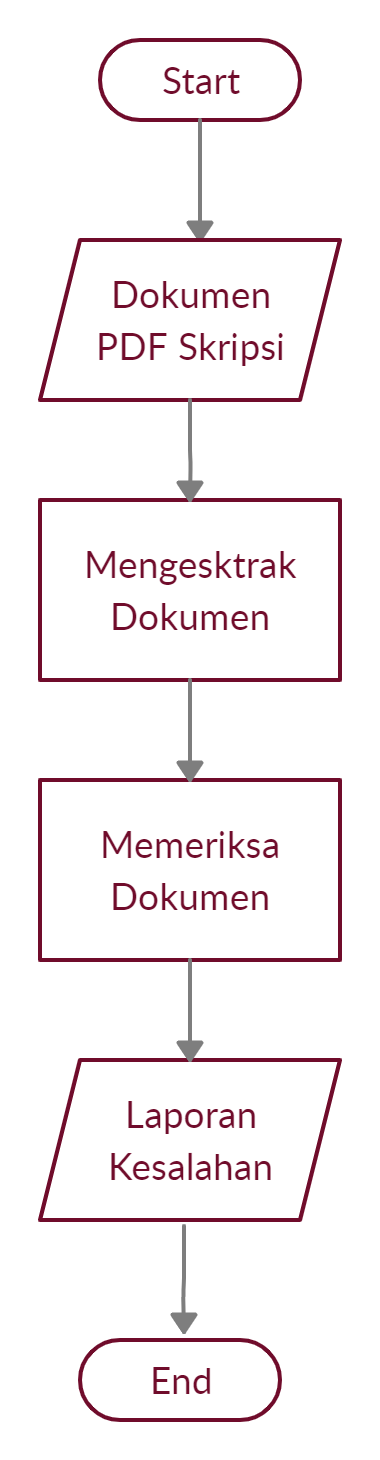
\includegraphics[scale=0.24]{flow-chart.png}
	\caption{Flow Chart Aplikasi Pemeriksa Kesalahan Dokumen Skripsi}	
	\label{fig:flow-chart} 
\end{figure}

Gambar \ref{fig:flow-chart} merupakan proses yang dibutuhkan untuk dapat memeriksa dan menghasilkan laporan kesalahan dokumen. Penjelasan dari \textit{flow chart} di atas adalah sebagai berikut:

\begin{enumerate}
	\item Aplikasi akan menerima masukan berupa dokumen PDF skripsi Informatika UNPAR dengan mode \textit{final}. Aplikasi akan mengambil nama dari dokumen beserta lokasi dari dokumen tersebut.
	
	\item Tahap kedua adalah mengekstrak dokumen PDF skripsi. Pada tahap ini, aplikasi akan menggunakan \textit{library Pdf Parser} untuk mengesktrak dokumen PDF skripsi. Dokumen skripsi akan diekstrak menjadi beberapa bagian, seperti halaman cover, daftar isi, bab, daftar pustaka dan lain-lain. Hasil ekstrak dari setiap bagian-bagian tersebut akan disimpan dalam sebuah string. Jumlah string yang tersedia bergantung dengan jumlah konten yang akan digunakan. Untuk mempermudah proses pemeriksaan, setiap string akan dipecah menjadi kalimat-kalimat yang disimpan dalam struktur data \textit{Array} 1 dimensi.
	
	\item Tahap ketiga adalah memeriksa kesalahan pada dokumen skripsi. Pada skripsi ini, fitur kesalahan yang telah diseleksi berjumlah 8 buah. Setiap fitur akan memiliki tugasnya masing-masing dalam mencari kesalahan. Setiap fitur pemeriksa akan memeriksa kesalahan menggunakan pencocokan pola dengan \textit{regular expression}. Pemeriksa akan mencocokan pola dengan kalimat-kalimat yang sudah disimpan \textit{array}. Misalnya, fitur pemeriksa kelengkapan data skripsi akan memeriksa array yang berisi halaman cover saja.
	
	\item Tahap terakhir adalah mengeluarkan laporan kesalahan pada dokumen skripsi. Pada tahap ini, laporan kesalahan akan ditampilkan secara terurut dan sekaligus setelah aplikasi dijalankan. Format laporan yang dikeluarkan meliputi kode kesalahan, jenis kesalahan dan bagian yang terdapat kesalahan. Laporan kesalahan akan dikeluarkan pada terminal.
\end{enumerate}